%%!TEX root = all.tex
%arrays --- YES
%arXiv
\chapter{Kirszbraun revisited}

This chapter is based on our paper \cite{akp-kirszbraun}
and earlier paper of Urs Lang and  Viktor Schroeder
\cite{lang-schroeder}.


\section{Short map extension definitions.}\label{sec:4pt}

\begin{thm}{Theorem}\label{thm:kirsz-def} 
Acomplete length space
$\spc{L}$ is $\Alex\kappa$ if and only if for any 3-point set $V_3$ and any 4-point set $V_4\supset V_3$ in $\spc{L}$, 
any short map $f\:V_3\to\Lob2\kappa$ can be extended to a short map $F\:V_4\to\Lob2\kappa$ (so $f=F|_{V_3}$).
\end{thm}

The proof of the ``only if'' part of Theorem \ref{thm:kirsz-def} can be obtained as a corollary of Kirszbraun's theorem (\ref{thm:kirsz+}).
We present another, more elementary proof; it use the following analog of Alexandrov lemma (\ref{lem:alex}).

We say that  two triangles with a common vertex  \index{overlap}\emph{do not overlap} if their convex hulls intersect only at the common vertex.


\begin{thm}{Overlap lemma}\label{lem:extend-overlap}
Let $\trig{\tilde x^1}{\tilde x^2}{\tilde x^3}$ be a triangle in $\Lob2{\kappa}$.  Let $\tilde p^1,\tilde p^2,\tilde p^3$ be points such that, for any permutation $\{i,j,k\}$ of $\{1,2,3\}$, we have
\begin{enumerate}[(i)]

\item 
\label{no-overlap:px=px}
$\dist{\tilde p^i}{\tilde x^\kay}{}=\dist{\tilde p^j}{\tilde x^\kay}{}$,
%$\dist{\tilde p^i}{\tilde x^\kay}{}=\dist{\tilde p^j}{\tilde x^\kay}{}$,

\item
\label{no-overlap:orient-1}
$\tilde p^i$ and $\tilde x^i$ lie in the same closed halfspace determined by $[\tilde x^j\tilde x^\kay]$,  
\end{enumerate}

Assume no pair of triangles $\trig{\tilde p^i}{\tilde x^j}{\tilde x^\kay}$ overlap
then 
\[\mangle{\tilde p^1} +\mangle {\tilde p^2}+\mangle{\tilde p^3}> 2\cdot\pi,\]
where $\mangle\tilde p^i$ denotes $\mangle\hinge{\tilde p^i}{\tilde x^\kay}{\tilde x^j}$
for a permutation $\{i,j,k\}$ of $\{1,2,3\}$.
\end{thm}

\begin{wrapfigure}{r}{21mm}
\begin{lpic}[t(-0mm),b(0mm),r(0mm),l(0mm)]{pics/contr-no-overlap(1)}
\lbl[lt]{12,15.5;{\small $\tilde p^1$}}
\lbl[bl]{5.5,18;{\small $\tilde p^2$}}
\lbl[r]{5,6.5;{\small $\tilde p^3$}}
\lbl[lb]{4,25;$\tilde x^1$}
\lbl[t]{2,0;$\tilde x^2$}
\lbl[l]{18,16;$\tilde x^3$}
\end{lpic}
\end{wrapfigure}

\parbf{Remarks.}
If $\kappa\le 0$, then overlap lemma can be proved without using condition (\ref{no-overlap:px=px}).
This follows immediately from the formula that relates the sum of angles for the hexagon
$[\tilde p^1\tilde x^2\tilde p^3\tilde x^1\tilde p^2\tilde x^3]$ and its area:
\[ \mangle\tilde p^1
-
\mangle\tilde x^2
+
\mangle\tilde p^3
-
\mangle\tilde x^1
+
\mangle\tilde p^2
-
\mangle\tilde x^3
=2\cdot\pi-\kappa\cdot{\area}.
\]

The diagram shows that condition (\ref{no-overlap:px=px}) is essential
in case $\kappa>0$.

                            




\parit{Proof.}   Rotate the  triangle $\trig{\tilde p^3}{\tilde x^1}{\tilde x^2}$ around $\tilde x^1$ to make $[\tilde x^1\tilde p^3]$ coincide with $[\tilde x^1\tilde p^2]$.
Let  $\dot x^2$ denote the image of $\tilde x^2$ after rotation. 
Note that 
$$\mangle\hinge{\tilde x^1}{\tilde x^3}{\dot x^2}
=
\min\{\,\mangle\hinge {\tilde x^1}{\tilde x^2}{\tilde p^3}
+
\mangle\hinge {\tilde x^1}{\tilde p^2}{\tilde x^3},\,
2\cdot\pi -(\mangle\hinge {\tilde x^1}{\tilde x^2}{\tilde p^3}
+
\mangle\hinge {\tilde x^1}{\tilde p^2}{\tilde x^3})\,\}.
$$
By (\ref{no-overlap:orient-1}), 
the triangles 
$\trig{\tilde p^3}{\tilde x^1}{\tilde x^2}$ 
and $\trig{\tilde p^2}{\tilde x^3}{\tilde x^1}$ do not overlap if and only if 
\[
2\cdot\pi>\mangle\hinge {\tilde x^1}{\tilde x^2}{\tilde p^3}+\mangle\hinge {\tilde x^1}{\tilde p^2}{\tilde x^3}+\mangle\hinge {\tilde x^1}{\tilde x^2}{\tilde x^3}\eqlbl{eq:old-iii}\]
and
\[\mangle\hinge{\tilde x^1}{\tilde x^3}{\tilde x^2}
> 
\mangle\hinge{\tilde x^1}{\tilde x^3}{\dot x^2}.\eqlbl{eq:main-overlap}\]
The condition \ref{eq:main-overlap} holds if and only if 
$\dist{\tilde x^2}{\tilde x^3}{}>\dist{\dot x^2}{\tilde x^3}{}$,
which in turn holds if and only if 
\[
\begin{aligned}
\mangle\tilde p^1
&> \mangle\hinge{\tilde p^2}{\tilde x^3}{\dot x^2}
\\
&=
\min\{\mangle\tilde p^3+\mangle\tilde p^2,2\cdot\pi -(\mangle\tilde p^3+\mangle\tilde p^2)\}.
\end{aligned}
\eqlbl{eq:no-overlap}\]
The  inequality follows since the  corresponding hinges have the same pairs of sidelengths.
(The two pictures show that both possibilities for the minimum can occur.)

\begin{center} 
%\begin{wrapfigure}{l}{44mm} 
\begin{lpic}[t(0mm),b(0mm),r(0mm),l(0mm)]{pics/4-pnt-kirsz-x2(1)}
\lbl[br]{13.5,7;{\small $\tilde p^3$}}
\lbl[t]{17,12.5;{\small $\tilde p^1$}}
\lbl[bl]{8,14;{\small $\tilde p^2$}}
\lbl[t]{1,0;$\tilde x^1$}
\lbl[t]{29,0;$\tilde x^2$}
\lbl[b]{22.5,22;$\dot x^2$}
\lbl[b]{10,36;$\tilde x^3$}
%\end{lpic}
%\begin{lpic}[t(5mm),b(0mm),r(0mm),l(0mm)]{pics/4-pnt-kirsz-sba(0.4)}
\lbl[rt]{61,9;{\small $\tilde p^1$}}
\lbl[l]{76,22;$\tilde p^2$}
\lbl[l]{81,7;$\tilde p^3$}
\lbl[t]{42,0;$\tilde x^1$}
\lbl[t]{70,0;$\tilde x^2$}
\lbl[lt]{68,13;$\dot x^2$}
\lbl[b]{50,36;$\tilde x^3$}
\end{lpic}       


%\end{wrapfigure}
\end{center}

Now assume $\mangle\tilde p^1 + \mangle\tilde p^2+\mangle\tilde p^3 \le 2\cdot\pi$.
Then  \ref{eq:no-overlap} implies 
\[\mangle\tilde p^i>\mangle\tilde p^j + \mangle\tilde p^\kay.\]
Since no pair of triangles overlap, the same holds 
for any permutation $(i,j,\kay)$ of $(1,2,3)$.
Therefore
\[\mangle\tilde p^1+\mangle\tilde p^2+\mangle\tilde p^3>2\cdot(\mangle\tilde p^1+\mangle\tilde p^2+\mangle\tilde p^3),\]
a contradiction. 
\qeds

\parit{Proof of \ref{thm:kirsz-def}; ``if'' part.} 
Assume $\spc{L}$ is geodesic.
Take $x^1,x^2,x^3\in \spc{L}$ so the model triangle 
$\trig{\tilde x^1}{\tilde x^2}{\tilde x^3}=\modtrig\kappa(x^1 x^2 x^3)$ is defined.
Choose $p\in \,{]}x^1x^2{[}\,$;
apply Kirszbrun property for $V_3=\{x^1,x^2,x^3\}$ and 
$V_4=\{x^1,x^2,x^3,p\}$ and the map $f(x^i)=\tilde x^i$. 
You obtain point-on-side comparison (\ref{point-on-side}).

In case $\spc{L}$ is not geodesic, pass to its ultrapower $\spc{L}^\o$.
Note that the short map extension property survives
for $\spc{L}^\o$ and recall that $\spc{L}^\o$ is geodesic (see \ref{cor:ulara-geod}).
Thus, from above, $\spc{L}^\o$ is a complete length $\Alex\kappa$ space. 
By Proposition~\ref{prp:A^omega}, $\spc{L}$ is a complete length $\Alex\kappa$ space.

\parit{``Only if'' part.}
Assume the contrary;
that is,  $x^1,x^2,x^3,p\in \spc{L}$, and 
$\tilde x^1,\tilde x^2,\tilde x^3\in\Lob2\kappa$ are such that
$\dist{\tilde x^i}{\tilde x^j}{}\le\dist{x^i}{x^j}{}$ for all $i,j$ and there is no point $\tilde p\in \Lob2\kappa$ such that $\dist{\tilde p}{\tilde x^i}{}\le \dist{p}{x^i}{}$ for all $i$.

Note that in this case all comparison triangles $\modtrig\kappa(p x^ix^j)$ are defined.
That is always true if $\kappa\le0$.
If $\kappa>0$, and say $\modtrig\kappa(p x^1x^2)$ is undefined, then 
\begin{align*}
\dist{p}{x^1}{}+\dist{p}{x^2}{}
&\ge 2\cdot\varpi\kappa-\dist{x^1}{x^2}{}
\ge
\\
&\ge
2\cdot\varpi\kappa-\dist{\tilde x^1}{\tilde x^2}{}\ge 
\\
&\ge 
\dist{\tilde x^1}{\tilde x^3}{}+\dist{\tilde x^2}{\tilde x^3}{}.
\end{align*}
It follows that we can take $\tilde p$ on $[\tilde x^1\tilde x^3]$ or  $[\tilde x^2\tilde x^3]$.

For each $i\in \{1,2,3\}$, consider a point $\tilde p^i\in\Lob2\kappa$ such that $\dist{\tilde p^i}{\tilde x^i}{}$ is minimal among points satisfying $\dist{\tilde p^i}{\tilde x^j}{}\le\dist{p}{ x^j}{}$ for all $j\not=i$. 
Clearly, every $\tilde p^i$ is inside the triangle $\trig{\tilde x^1}{\tilde x^2}{\tilde x^3}$ (that is, in $\Conv(\tilde x^1,\tilde x^2,\tilde x^3)$), and $\dist{\tilde p^i}{\tilde x^i}{}>\dist{p}{ x^i}{}$ for each $i$.
Since the function $x\mapsto\tangle\mc\kappa\{x;a,b\}$
is increasing, it follows that
\begin{enumerate}[(i)]
\item $\dist{\tilde p^i}{\tilde x^j}{}=\dist{p}{ x^j}{}$ for $i\not=j$;
\item no pair of triangles from $\trig{\tilde p^1}{\tilde x^2}{\tilde x^3}$, $\trig{\tilde p^2}{\tilde x^3}{\tilde x^1}$, $\trig{\tilde p^3}{\tilde x^1}{\tilde x^2}$ overlap in $\trig{\tilde x^1}{\tilde x^2}{\tilde x^3}$.
\end{enumerate}

As follows from the overlap lemma (\ref{lem:extend-overlap}), 
in this case 
\[\mangle\hinge {\tilde p^1}{\tilde x^2}{\tilde x^3} 
+\mangle\hinge {\tilde p^2}{\tilde x^3}{\tilde x^1}
+\mangle\hinge {\tilde p^3}{\tilde x^1}{\tilde x^2}
>2\cdot\pi.
\]
Since $\dist{\tilde x^i}{\tilde x^j}{}\le\dist{x^i}{x^j}{}$ we get
\[\mangle\hinge {\tilde p^\kay}{\tilde x^i}{\tilde x^j}
\le
\angk\kappa p{x^i}{x^j}\]
if $(i,j,k)$ is a permutation of $(1,2,3)$.
Therefore 
\[\angk\kappa p{x^1}{x^2}+\angk\kappa p{x^2}{x^3}+\angk\kappa p{x^3}{x^1}>2\cdot\pi;\]
the later contradicts $\Alex\kappa$ comparison (\ref{df:cbb1+3}).
\qeds

\begin{thm}{Theorem}\label{thm:cba-kirsz-def} 
Assume any pair of points at distance $<\varpi\kappa$ in the metric space $\spc{U}$ are joined by a unique geodesic. 
Then $\spc{U}$ is $\CAT\kappa$ if and only if 
for any $3$-point set $V_3$  with perimeter $<2\cdot\varpi\kappa$
and any $4$-point set $V_4\supset V_3$ in $\Lob2\kappa$, 
any short map $f\:V_3\to\spc{U}$ can be extended to a short map $F\:V_4\to\spc{U}$.
\end{thm}

Note that the ``only if'' part of Theorem \ref{thm:cba-kirsz-def} does not follow directly from Kirszbraun's theorem, since the desired extension is in $\spc{U}$ --- not its completion.

\begin{thm}{Lemma}\label{lem:smaller-trig}
Let $x^1,x^2,x^3,y^1,y^2,y^3\in\Lob{}{\kappa}$
be points such that $\dist{x^i}{x^j}{}\ge\dist{y^i}{y^j}{}$ for all $i,j$.
Then there is a short map $\map\:\Lob{}{\kappa}\to\Lob{}{\kappa}$ such that $\map(x^i)=y^i$ for all $i$;
moreover, one can choose $\map$ so that 
\[\Im \map\subset\Conv(y^1,y^2,y^3).\]

\end{thm}

We only give an idea of the proof of  this lemma;
alternatively, one can get the result as a corollary of  Kirszbraun's theorem (\ref{thm:kirsz+}) 

\parit{Idea of the proof.}
The map $\map$ can be constructed as a composition of an isometry of $\Lob{}{\kappa}$ and the following folding maps:
Given a halfspace $H$ in $\Lob{}{\kappa}$, consider the map $\Lob{}{\kappa}\to H$, 
that is identity on $H$ and reflects all points outside of $H$ into $H$.
This map is a path isometry, in particular it is short. 

The last part of the lemma can be proved by composing the constructed map with foldings along the sides of triangle $\trig{y^1}{y^2}{y^3}$ and passing to a partial limit.
\qeds

\parit{Proof of \ref{thm:cba-kirsz-def}; ``if'' part.}
The point-on-side comparison (\ref{cat-monoton}) follows  by
taking $V_3=\{\tilde x,\tilde y,\tilde p\}$ and  $V_4=\{\tilde x,\tilde y,\tilde p,\tilde z\}$ where $z\in \mathopen{]}x y\mathclose{[}$.  
It is only necessary to observe that  $F(\tilde z)=z$ by uniqueness of $[x y]$.


\parit{``Only if'' part.}
Let $V_3=\{\tilde x^1,\tilde x^2,\tilde x^3\}$ and $V_4=\{\tilde x^1,\tilde x^2,\tilde x^3,\tilde p\}$.

Set $y^i\z=f(\tilde x^i)$ for all $i$;
we need to find a point $q\in\spc{U}$ such that $\dist{y^i}{q}{}\le\dist{\tilde x^i}{\tilde p}{}$ for all $i$.

Let $D$ be the convex set in $\Lob2\kappa$ bounded by the model triangle 
$\trig{\tilde y^1}{\tilde y^2}{\tilde y^3}\z=\modtrig\kappa{y^1}{y^2}{y^3}$;
that is, $D\z=\Conv({\tilde y^1},{\tilde y^2},{\tilde y^3})$.

Note that $\dist{\tilde y^i}{\tilde y^j}{}=\dist{y^i}{y^j}{}\le\dist{\tilde x^i}{\tilde x^j}{}$ for all $i,j$.
Applying Lemma \ref{lem:smaller-trig},
we get a short map 
$\map\:\Lob{}{\kappa}\to D$ such that 
$\map\:\tilde x^i\mapsto\tilde y^i$.

Further, by the majorization theorem (\ref{thm:major}), 
there is a short map $F\:D\to \spc{U}$ such that $\tilde y^i\mapsto y^i$ for all $i$.

Thus one can take $q=F\circ\map(\tilde p)$.
\qeds

\begin{thm}{Exercise}\label{ex:CBB+CBA}
Assume $\spc{X}$ is a complete length space that satisfies the following condition:
any 4-point subset can be isometrically embedded in Euclidean 3-space.

Prove that $\spc{X}$ is isometric to a closed convex substet of a Hilbert space.
\end{thm}

\begin{thm}{Exercise}\label{ex:5-point-CBA=>CBB}
Let $\spc{F}_s$ be the metric
on the 5 point set $\{p,q,x,y,z\}$ such that $\dist{p}{q}{}=s$
and all the remaining distances are equal $1$.
For which values $s$ the space $\spc{F}_s$ admits a distance preserving map into 
\begin{subthm}{}
a complete length $\CAT{0}$ space?
\end{subthm}
\begin{subthm}{}
a complete length $\Alex{0}$ space?
\end{subthm}
\end{thm}

\section{(1+\textit{n})-point comparison}\label{sec:1+n}

The following theorem gives a more sensitive analog of  $\Alex\kappa$ comparison (\ref{df:cbb1+3}).

\begin{thm}{(1+\textit{n})-point comparison}
\label{thm:pos-config} {\sloppy 
Let $\spc{L}$ be a complete length $\Alex{\kappa}$ space.
Then for any array of points $p,x^1,\dots,x^n\in \spc{L}$  
there is a model array $\tilde p,\tilde x^1,\dots,\tilde x^n\in\Lob{n}\kappa$ such that

}

\begin{subthm}{}
$\dist{\tilde p}{\tilde x^i}{}=\dist{p}{x^i}{}$ for all $i$.
\end{subthm}

\begin{subthm}{}$\dist{\tilde x^i}{\tilde x^j}{}\ge\dist{x^i}{x^j}{}$ for all $i,j$.
\end{subthm}
\end{thm}

\parit{Proof.} 
It is sufficient to show that given $\eps>0$ there is a configuration $\tilde p,\tilde x^1,\dots,\tilde x^n\in\Lob{n}\kappa$ such that 
\[\dist{\tilde x^i}{\tilde x^j}{}\ge\dist{x^i}{x^j}{}
\quad
\text{and}
\quad
\bigl|\dist{\tilde p}{\tilde x^i}{}-\dist{p}{x^i}{}\bigr|\le \eps.\]
Then one can pass to a limit configuration for $\eps\to 0+$.

According to \ref{thm:almost.geod}, the set $\Str(x^1,\dots,x^n)$ 
 is dense in $\spc{L}$.
Thus, there is a point $p'\in \Str(\tilde x^1,\dots,\tilde x^n)$ such  that $\dist{p'}{p}{}\le\eps$.
According to Corollary~\ref{cor:euclid-subcone}, 
$\T_{p'}$ contains a subcone $E$ isometric to a Euclidean space 
that contains all vectors $\ddir{p'}{x^i}$.
Passing to subspace if necessary, we can assume that $\dim E\le n$.

Mark a point $\tilde p\in \Lob{n}\kappa$ and choose a distance preserving map
$\iota\: E\to \T_{\tilde p}\Lob{n}\kappa$.
Set 
\[\tilde x^i
=
\exp_{\tilde p}\circ\iota(\ddir{p'}{x^i}).\]
Thus $\dist{\tilde p}{\tilde x^i}{}=\dist{p'}{x^i}{}$ and therefore
\[\bigl|\dist{\tilde p}{\tilde x^i}{}-\dist{p}{x^i}{}\bigr|
\le 
\dist{p}{p'}{} \le\eps.\]
From the hinge comparison (\ref{angle}) 
we have 
\[\angk\kappa{\tilde p}{\tilde x^i}{\tilde x^j}
=\mangle\hinge{\tilde p}{\tilde x^i}{\tilde x^j}
=\mangle\hinge{p'}{x^i}{x^j}\ge \angk\kappa{p'}{x^i}{x^j},\]
thus 
\[\dist{\tilde x^i}{\tilde x^j}{}\ge \dist{x^i}{x^j}{}.\]
\qedsf

\begin{thm}{Exercise}\label{ex:sturm}
Let $p,x_1,\dots,x_n$ be a point array in a $\Alex0$ space.
Consider the $n{\times}n$-matrix $M$ with the components 
\[m_{i,j}=\tfrac12\cdot(|x_i-p|^2+|x_j-p|^2-|x_i-x_j|^2).\]
Show that
\[\bm{s}\cdot M\cdot \bm{s}^\top\ge 0\eqlbl{eq:sMs}\]
for any vector $\bm{s}=(s_1,\dots,s_n)$ with nonnegative components.
\end{thm}

\begin{wrapfigure}{r}{22 mm}
\vskip-0mm
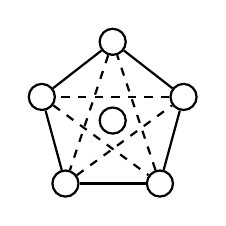
\begin{tikzpicture}[scale=1,
  thick,main node/.style={circle,draw,font=\sffamily\bfseries,minimum size=3mm}, ]

    \node[main node] (0) at (0,0){};
     \node[main node] (1) at (.6,-.8) {};
     \node[main node] (2) at (.9,.3){};
     \node[main node] (3) at (0,1) {};
  \node[main node] (4) at (-.9,.3) {};
  \node[main node] (5) at (-.6,-.8) {};

  \path[every node/.style={font=\sffamily\small}]
  (1) edge node[above]{}(2)
  (2) edge node[above]{}(3)
  (3) edge node[above]{}(4)
  (4) edge node[above]{}(5)
  (5) edge node[above]{}(1)
  (1) edge[dashed] node[above]{}(3)
  (2) edge[dashed] node[above]{}(4)
  (3) edge[dashed] node[above]{}(5)
  (4) edge[dashed] node[above]{}(1)
  (5) edge[dashed] node[above]{}(2);
\end{tikzpicture}
\end{wrapfigure}

The inequality in the above exercise is discovered by  Karl-Theodor Sturm \cite{sturm}.
It turns out to be weaker than (1+\textit{n})-point comparison.
An example can be constructed by perturbing the 6-point metric isometric to a regular pentagon with its center
by making its sides slightly longer and diagonals slightly shorter \cite{LPZ}.


\begin{thm}{Exercise}\label{ex:(3+1)-nonsufficient}
Give an example of metric on a finite set, that satisfies the comparison inequality 
\[\angk{0}{p}{x_1}{x_2}+\angk{0}{p}{x_2}{x_3}+\angk{0}{p}{x_3}{x_1}
\le
2\cdot\pi\]
for any quadruple of points $(p,x_1,x_2,x_3)$, 
but is not isometric to a subset of Alexandrov space with curvature $\ge0$.
\end{thm}

\begin{thm}{Exercise}\label{ex:strut+embedding}
Let $\spc{L}$ be a complete length $\Alex{\kappa}$ space. 
Assume that a point array $(a^0,a^1,\dots,a^\kay)$ in $\spc{L}$
 is \emph{$\kappa$-strutting} for a point $p\in\spc{L}$.
Show that there are point 
$\tilde p,\tilde a^0,\dots,\tilde a^m\in \Lob{m+1}\kappa$ such that
\[\dist{\tilde p}{\tilde a^i}{}=\dist{p}{a^i}{}\ \text{and}\ \dist{\tilde a^i}{\tilde a^j}{}=\dist{a^i}{a^j}{}\]
for all $i$ and $j$.
\end{thm}


\section{Helly's theorem}\label{sec:helly}

%???CHECK lang-schroeder HAlly THEOREM???

\begin{thm}{Helly's theorem}\label{thm:helly}
Let $\spc{U}$  be a complete length $\CAT0$ space
and $\{K_\alpha\}_{\alpha\in \IndexSet}$ be an arbitrary collection of closed bounded convex subsets of $\spc{U}$.

If 
\[\bigcap_{\alpha\in \IndexSet}K_\alpha=\emptyset\]
then there is an index array $\alpha_1,\alpha_2,\dots,\alpha_n\in \IndexSet$ such that
\[\bigcap_{i=1}^nK_{\alpha_i}=\emptyset.\]

%???Moreover, if $\dim \spc{U}\le m$, then one can assume above $n\le m+1$.
\end{thm}

\parbf{Remarks.}
\begin{enumerate}[(i)]
\item In general, none of $K_\alpha$ might be compact; 
otherwise the statement is trivial.
\item If $\spc{U}$ is a Hilbert space (not necessarily separable), 
then the above result is equivalent to the following statement: if a convex bounded set is closed in ordinary topology then it compact in the weak topology.
One can define \emph{weak topology} on arbitrary metric space, by taking exteriors of closed ball as its prebase.
Then the result above implies analogous statement for complete length $\CAT0$ spaces
(compare to \cite{monod}).
\end{enumerate}

\medskip

We present the original proof of Urs Lang and Viktor Schroeder from \cite{lang-schroeder}.

%\parit{Proof.}
%Let us first prove uniqueness. 
%Assume there are two points $y',y''\in K$ 
%so that $\dist{y'}{p}{}=\dist{y''}{p}{}=\dist{K}{p}{}$.
%Take $z$ to be midpoint of $[y'y'']$. 
%Since $K$ is convex, $z\in K$.
%From comparison, we have that $\dist{z}{p}{}<\dist{y'}{p}{}=\dist{K}{p}{}$, a contradiction
%
%The proof of existence is analogous.
%Take a sequence  of points $y_n\in K$ 
%such that $\dist{y_n}{p}{}\to \dist{K}{p}{}$.
%It is sufficient to show that $(y_n)$ converges in itself; 
%thus one could take $p^*=\lim_n y_n$.

%Assume $(y_n)$ does not converge in itself, then for some fixed $\eps>0$, 
%we can choose two subsequences $(y_n')$ and $(y_n'')$ of $(y_n)$ 
%such that 
%$\dist{y'_n}{y''_n}{}\ge\eps$ for each $n$.
%Set $z_n$ to be the midpoint of $[y'_ny''_n]$; from convexity we have $z_n\in K$.
%From point-on-side comparison \ref{cat-monoton}, there is $\delta>0$ 
%such that $\dist{p}{z_n}{}\le \max\{\dist{p}{y'_n}{},\dist{p}{y''_n}{}\}-\delta$. 
%Thus 
%\[\limsup_{n\to\infty}\dist{p}{z_n}{}<\dist{K}{x}{},\] 
%a contradiction\qeds

\parit{Proof of \ref{thm:helly}.} 
Assume the contrary. Then for any finite set $F\subset \IndexSet$
\[K_{F}\df \bigcap_{\alpha\in F}K_{\alpha}\not=\emptyset,\]
we will construct point $z$ such that $z\in K_\alpha$ for each $\alpha$.
Thus we will arrive to contradiction since
\[\bigcap_{\alpha\in \IndexSet}K_\alpha=\emptyset.\]

Choose a point $p\in \spc{U}$ and set $r=\sup\dist{K_{F}}{p}{}$ where $F$ runs all finite subsets of $\IndexSet$.
Set $p^*_F$ to be the closest point on $K_{F}$ from $p$; 
according to closest-point projection lemma (\ref{lem:closest point}), $p^*_F$ 
exits and is unique.

Take a nested sequence of finite subsets 
$F_1\subset F_2\subset \dots$ of $\IndexSet$, such that $\dist{K_{F_n}}{p}{}\to r$.

Let us show that the sequence $(p^*_{F_n})$ converges in itself. 
Indeed, if not, then for some fixed $\eps>0$, 
we can choose two subsequences $(y'_n)$ and $(y''_n)$ of $(p^*_{F_n})$ 
such that $\dist{y'_n}{y''_n}{}\ge\eps$.
Set $z_n$ to be midpoint of $[y'_ny''_n]$. 
From point-on-side comparison (\ref{point-on-side}), 
there is $\delta>0$ such that 
\[\dist{p}{z_n}{}\le \max\{\dist{p}{y'_n}{},\dist{p}{y''_n}{}\}-\delta.\]
Thus 
\[\limsup_{n\to\infty}\dist{p}{z_n}{}<r.\]
On the other hand, from convexity, each $F_n$ 
contains all $z_\kay$ with sufficiently large $\kay$, a contradiction.

Thus, $p^*_{F_n}$ converges and we can set $z=\lim_n p^*_{F_n}$.
Clearly 
\[\dist{p}{z}{}=r.\]

Repeat the above arguments for  the sequence $F_n'=F_n\cup \{\alpha\}$.
As a result, we get another point $z'$ such that $\dist{p}{z}{}=\dist{p}{z'}{}=r$ and 
$z,z'\in K_{F_n}$ for all $n$.
Thus, if $z\not=z'$ the midpoint $\hat z$ of $[zz']$ would belong to all 
$K_{F_n}$ and from comparison we would have $\dist{p}{\hat z}{}<r$, a contradiction.

Thus, $z'=z$; in particular 
$z\in K_\alpha$ for each $\alpha\in\IndexSet$.
\qeds



\section{Kirszbraun's theorem}\label{sec:kirszbraun}

A slightly weaker version of the following theorem was proved by Urs Lang and Viktor Schroeder \cite{lang-schroeder}.

\begin{thm}{Kirszbraun's theorem}
\label{thm:kirsz+}
Let
$\spc{L}$ be a complete length $\Alex{\kappa}$ space, 
$\spc{U}$ be a complete length $\CAT\kappa$ space, 
$Q\subset \spc{L}$ be arbitrary subset
and $f\: Q\to\spc{U}$ be a short map.
Assume that there is $z\in\spc{U}$ such that 
$f(Q)\subset \oBall[z,\tfrac{\varpi\kappa}{2}]_{\spc{U}}$.
Then $f\:Q\to\spc{U}$ can be extended to a short map 
$F\:\spc{L}\to \spc{U}$
(that is, there is a short map $F\:\spc{L}\to \spc{U}$ such that $F|_Q=f$.)
\end{thm}
 
The condition $f(Q)\subset \oBall[z,\tfrac{\varpi\kappa}{2}]$ trivially holds for any $\kappa\le 0$ since in this case $\varpi\kappa=\infty$. 
The following example shows that this condition is needed for $\kappa>0$.

The Conjecture~\ref{conj:kirsz} (if true) gives an equivalent condition for the existence of a short extension;
roughly it states the following example is the only obstacle.

\begin{thm}{Example}\label{example:SS_+}
Let $\mathbb{S}^m_+$ be a closed $m$-dimensional unit hemisphere.  Denote its boundary, which is isometric to $\mathbb{S}^{m-1}$, by  $\partial\mathbb{S}^m_+$.
Clearly, $\mathbb{S}^m_+$ is $\Alex{1}$ and $\partial\mathbb{S}^m_+$ is $\CAT1$, but the identity map ${\partial\mathbb{S}^m_+}\to \partial\mathbb{S}^m_+$ cannot be extended to a short map $\mathbb{S}^m_+\to \partial\mathbb{S}^m_+$ (there is no place for the pole).

There is also a direct generalization of this example to a hemisphere in a Hilbert space of arbitrary cardinal dimension.
\end{thm}

First we prove this theorem in the case $\kappa\le 0$ (\ref{thm:kirsz}).
In the proof of the more complicated case $\kappa>0$, we use the case $\kappa=0$.
The following lemma is the main ingredient in the proof. 

\begin{thm}{Finite$\bm{+}$one lemma}\label{lem:kirsz-neg:new}
Let $\kappa\le 0$,
$\spc{L}$ be a complete length $\Alex{\kappa}$ space, and 
$\spc{U}$ be a complete length $\CAT\kappa$ space.
Suppose
$x^1,x^2,\dots,x^n\in\spc{L}$ 
and $y^1,y^2,\dots,y^n\in\spc{U}$
are
such that $\dist{x^i}{x^j}{}\ge\dist{y^i}{y^j}{}$ for all $i,j$.

Then for any $p\in\spc{L}$, there is $q\in\spc{U}$ such that $\dist{y^i}{q}{}\le\dist{x^i}{p}{}$ for each $i$.
\end{thm}

\parit{Proof.}
It is sufficient to prove the lemma only for $\kappa=0$ and $-1$.
The proofs of these two cases are identical, only the formulas differ.
In the proof, we assume $\kappa=0$ and provide the formulas for $\kappa=-1$ in the footnotes.

From (1+\textit{n})-point comparison (\ref{thm:pos-config}), 
there is a model configuration 
$\tilde p,\tilde x^1,\tilde x^2,\dots,\tilde x^n\in \Lob{n}{\kappa}$ such that
$\dist{\tilde p}{\tilde x^i}{}=\dist{p}{x^i}{}$
and $\dist{\tilde x^i}{\tilde x^j}{}\ge\dist{x^i}{x^j}{}$ 
for all $i$, $j$.
It follows that we can assume that $\spc{L}=\Lob{n}{\kappa}$.

For each $i$, consider functions 
$f^i\:\spc{U}\to\RR$ and $\tilde f^i\:\Lob{n}{\kappa}\to\RR$ 
defined as follows%
%%%%%%%%%%%%
\footnote{In case $\kappa=-1$,
\[
\begin{aligned}
&f^i=\cosh\circ\distfun{y^i}{}{},
&
&\tilde f^i=\cosh\circ\distfun{\tilde x^i}{}{}.
\end{aligned}
\leqno{(A)\mc-}\]}
%%%%%%%%%%%%
\[
\begin{aligned}
&f^i=\tfrac{1}{2}\cdot\distfun[2]{y^i}{}{},
&
&\tilde f^i=\tfrac{1}{2}\cdot\distfun[2]{\tilde x^i}{}{}.
\end{aligned}
\leqno{(A)\mc0}
\]
Set
$\bm{f}=(f^1,f^2,\dots,f^n)\:\spc{U}\to\RR^n$ and $\bm{\tilde f}=(\tilde f^1,\tilde f^2,\dots,\tilde f^n)\:\Lob{n}{\kappa}\to\RR^n$.

Recall that the set $\Up\bm{f}(\spc{U})\subset\RR^n$ is defined on page \pageref{PAGE.def:Up}.
Note that it is sufficient to prove that
$\bm{\tilde f}(\tilde p)\in\Up\bm{f}(\spc{U})$.

Clearly,
$(f^i)''\ge 1$.
Thus, by the theorem on barycentric simplex (\ref{thm:web:Up-convex}), 
the set $\Up\bm{f}(\spc{U})\subset\RR^{n}$ is convex.

Arguing by contradiction, let us assume that $\bm{\tilde f}(\tilde p)\notin\Up\bm{f}(\spc{U})$.

Then there  exists a supporting hyperplane  $\alpha_1\cdot x_1+\ldots \alpha_n\cdot x_n=c$ to $\Up\bm{f}(\spc{U})$, separating it from  $\bm{\tilde f}(\tilde p)$.
According to Lemma~\ref{lem:Up-convex:subnormal}, 
$\alpha_i\ge 0$ for each $i$. 
So we can assume that $(\alpha_1,\alpha_2,\dots,\alpha_n)\in\Delta^{n-1}$
(that is, $\alpha_i\ge 0$ for each $i$ and $\sum\alpha_i=1$)
and 
\[\sum_i\alpha_i\cdot\tilde f^i(\tilde p)
< 
\inf
\set{\sum_i\alpha_i\cdot f^i(q)}{q\in\spc{U}}.\]
The latter contradicts the following claim.

\begin{clm}{}
Given $\bm{\alpha}=(\alpha_1,\alpha_2,\dots,\alpha_n)\in\Delta^{n-1}$,
set
\begin{align*}
&h=\sum_i\alpha_i\cdot f^i
&
&h\:\spc{U}\to\RR
&
&z=\argmin h\in \spc{U}
\\
&\tilde h=\sum_i\alpha_i\cdot \tilde f^i
&
&\tilde h\:\Lob{n}{\kappa}\to\RR
&
&\tilde z=\argmin \tilde h\in \Lob{n}{\kappa}
\end{align*}
Then 
$h(z)\le \tilde h(\tilde z)$.
\end{clm}

\parit{Proof of the claim.}
Note that $\dd_z h\ge 0$.
Thus, for each $i$, we have%
\footnote{In case $\kappa=-1$, the same calculations give
\[
\begin{aligned}
0
&\le\dots \le
-\tfrac{1}{\sinh\dist[{{}}]{z}{y^i}{}}
\cdot 
\sum_j
\alpha_j\cdot\left[\cosh\dist[{{}}]{z}{y^i}{}\cdot\cosh\dist[{{}}]{z}{y^j}{}-\cosh\dist[{{}}]{y^i}{y^j}{}\right].
\end{aligned}
\leqno{(B)\mc-}
\]

}

\[
\begin{aligned}
0
&\le (\dd_z h)(\dir{z}{y^i})
=
\\
&=
-\sum_j\alpha_j\cdot\dist[{{}}]{z}{y^j}{}\cdot\cos\mangle\hinge{z}{y^i}{y^j}
\le
\\
&\le
-\sum_j\alpha_j\cdot\dist[{{}}]{z}{y^j}{}\cdot\cos\angk0{z}{y^i}{y^j}
=
\\
&=
-\tfrac{1}{2\cdot\dist[{{}}]{z}{y^i}{}}
\cdot 
\sum_j
\alpha_j\cdot\left[\dist[2]{z}{y^i}{}+\dist[2]{z}{y^j}{}-\dist[2]{y^i}{y^j}{}\right].
\end{aligned}
\leqno{(B)\mc0}\]
In particular%
%%%%%%%%%%
\footnote{In case $\kappa=-1$, the same calculations give
\[
\begin{aligned} 
\sum_{i}\alpha_i\cdot\left[\sum_j
\alpha_j\cdot\left[\cosh\dist[{{}}]{z}{y^i}{}\cdot\cosh\dist[{{}}]{z}{y^j}{}
-\cosh\dist[{{}}]{y^i}{y^j}{}\right]
\right]\le0
\end{aligned}.
\leqno{(C)\mc-}
\]
},
%%%%%%%%%%
\[
\begin{aligned}
\sum_{i}
\alpha_i
\cdot
\left[\sum_j
\alpha_j
\cdot
\left[\dist[2]{z}{y^i}{}+\dist[2]{z}{y^j}{}-\dist[2]{y^i}{y^j}{}\right]
\right]\le 0,
\end{aligned}
\leqno{(C)\mc0}
\]
or%
%%%%%%%%%%
\footnote{In case $\kappa=-1$,
\[(h(z))^2\le
\sum_{i,j}
\alpha_i\cdot\alpha_j
\cdot
\cosh\dist[{{}}]{y^i}{y^j}{}. \leqno{(D)\mc-}\]
}
%%%%%%%%%%
\[2\cdot h(z)
\le
\sum_{i,j}
\alpha_i\cdot\alpha_j
\cdot
\dist[2]{y^i}{y^j}. \leqno{(D)\mc0}\]

Note, that if $\spc{U}\iso\Lob{n}{\kappa}$, 
then all inequalities in $(B,C,D)$ are sharp.
Thus the same argument as above, repeated for $\tilde x^1,\tilde x^2,\dots,\tilde x^n\in\Lob{n}{\kappa}$
gives%
\footnote%
{In case $\kappa=-1$,
\[(\tilde h(\tilde z))^2
=
\sum_{i,j}
\alpha_i\cdot\alpha_j
\cdot
\cosh\dist[{{}}]{\tilde x^i}{\tilde x^j}{}.
\leqno{(E)\mc-}\]
}
\[
2\cdot \tilde h(\tilde z)
=
\sum_{i,j}
\alpha_i\cdot\alpha_j
\cdot
\dist[2]{\tilde x^i}{\tilde x^j}{}. 
\leqno{(E)\mc0}
\]
Note that 
\[\dist{\tilde x^i}{\tilde x^j}{}
\ge
\dist{x^i}{x^j}{}\ge\dist{y^i}{y^j}{}\]
for all $i$, $j$.
Thus, $(D)$ and $(E)$ imply the claim.
\qedqeds






\begin{thm}{Kirszbraun's theorem for nonpositive bound}
\label{thm:kirsz}
Let
$\kappa\le0$,
$\spc{L}$ be a complete length $\Alex{\kappa}$ space, 
$\spc{U}$ be a complete length $\CAT\kappa$ space, 
$Q\subset \spc{L}$ be arbitrary subset
and $f\: Q\to\spc{U}$ be a short map.
Then there is a short extension 
$F\:\spc{L}\to \spc{U}$ of $f$;
that is, there is a short map $F\:\spc{L}\to \spc{U}$ such that $F|_Q=f$.
\end{thm}

\parbf{Remark.}
If $\spc{U}$ is proper, then we do not need Helly's theorem (\ref{thm:helly}) --- compactness of closed balls in $\spc{U}$ is sufficient in this case.


\parit{Proof of \ref{thm:kirsz}.} 
By Zorn's lemma, we can assume 
that $Q\subset\spc{L}$ is a maximal set;
that is, $f\:Q\to\spc{U}$ does not admits a short extension to any larger set $Q'\supset Q$.

Let us argue by contradiction.
Assume that $Q\not=\spc{L}$;
choose $p\in \spc{L}\backslash Q$.
Then
\[\bigcap_{x\in Q} \cBall[f(x),\dist{p}{x}{}]
=
\emptyset.\]

Since $\kappa\le 0$, the balls are convex; 
thus, by Helly's theorem (\ref{thm:helly}), 
one can choose a point array $x^1,x^2,\dots, x^n\in Q$ such that
\[\bigcap_{i=1}^n \cBall[y^i,\dist{x^i}{p}{}]
=
\emptyset,
\eqlbl{eq:cap=cBalls=0}\]
where $y^i=f(x^i)$.
Finally note that \ref{eq:cap=cBalls=0} contradicts the Finite+one lemma (\ref{lem:kirsz-neg:new})\qeds




\parit{Proof of Kirszbraun's theorem (\ref{thm:kirsz+}).} 
The case $\kappa\le 0$ is already proved in \ref{thm:kirsz}.
Thus it remains to prove the theorem only in case $\kappa>0$.
After rescaling we may assume that $\kappa=1$
and therefore $\varpi\kappa=\pi$.

Since $\cBall[z,\pi/2]_{\spc{U}}$ is a complete length $\CAT\kappa$ space, we can assume $\spc{U}=\cBall[z,\pi/2]_{\spc{U}}$. 
In particular, $\diam\spc{U}\le\pi$.

Further, any two points $x,y\in \spc{U}$ such that $\dist{x}{y}{}<\pi$ are joined by a unique geodesic;
if $\dist{x}{y}{}=\pi$, then the concatenation  of 
$[x z]$ and $[z y]$ as a geodesic from $x$ to $y$.
Hence $\spc{U}$ is geodesic.

We can also assume that $\diam\spc{L}\le\pi$.
Otherwise $\spc{L}$ is one-dimensional (see \ref{diam-k>0});
in this case the result follows since $\spc{U}$ is geodesic.

\medskip

Assume the theorem is false. Then 
there is a set $Q\subset \spc{L}$, 
a short map $f\: Q\to \spc{U}$ and  
$p\in \spc{L}\backslash  Q$ such that 
\[\bigcap_{x\in  Q}
\cBall[f(x),\dist{x}{p}{}]=\emptyset.
\eqlbl{eq:cap-of-balls}\]

We will apply \ref{thm:kirsz} for $\kappa=0$ to Euclidean cones $\mathring{\spc{L}}=\Cone \spc{L}$ and $\mathring{\spc{U}}\z=\Cone \spc{U}$. 
Note that 
\begin{itemize}
\item ${\mathring{\spc{U}}}$ is a complete length $\CAT0$ space, %???(see ???)
\item since $\diam \spc{L}\le \pi$ we have ${\mathring{\spc{L}}}$ is $\Alex{0}$. %???(see ???).
\end{itemize}
Further, we will view spaces $\spc{L}$ and $\spc{U}$ as unit spheres in $\mathring{\spc{L}}$ and $\mathring{\spc{U}}$ respectively.
In the cones $\mathring{\spc{L}}$ and $\mathring{\spc{U}}$ we will use 
``$|{*}|$'' for distance to the vertex, denoted by $\0$, 
``$\cdot$'' for cone multiplication,
``$\mangle(x,y)$'' for $\mangle\hinge{o}{x}{y}$ 
and ``$\<x,y\>$'' for $|x|\cdot|y|\cdot\cos\mangle\hinge{o}{x}{y}$.
In particular,
\begin{itemize}
\item $\dist{x}{y}{\spc{L}}=\mangle(x,y)$ for any $x,y\in\spc{L}$,
\item $\dist{x}{y}{\spc{U}}=\mangle(x,y)$ for any $x,y\in\spc{U}$,
\item for any $y\in \spc{U}$, we have
\[\mangle(z,y)\le\tfrac\pi2.
\eqlbl{eq:=<pi/2}\]

\end{itemize}
Set $\mathring{Q}=\Cone Q\subset \mathring{\spc{L}}$ and let $\mathring f\:\mathring{Q}\to \mathring{\spc{U}}$ be the natural cone extension of $f$; 
that is, 
$y=f(x)$ $\Rightarrow$ $t\cdot y=\mathring f(t\cdot x)$ 
for $t\ge0$.
Clearly $\mathring f$ is short.

Applying \ref{thm:kirsz} for $\mathring f$, 
we get a short extension map $\mathring F\:\mathring{\spc{L}}\to\mathring{\spc{U}}$. 
Set $s=\mathring F(p)$.
Thus, 
\[\dist{s}{\mathring f(w)}{}
\le 
\dist{p}{w}{}
\eqlbl{eq:clm:kirszbraun-curv=1-rad-star}\]
for any $w\in \mathring Q$.
In particular, $|s|\le 1$.
Applying \ref{eq:clm:kirszbraun-curv=1-rad-star} 
for $w=t\cdot x$ and $t\to\infty$ we get

\[\<f(x),s\>\ge \cos\mangle(p,x)\eqlbl{eq:<,>=<}\]
for any $x\in Q$.

\begin{wrapfigure}{r}{33mm}
\begin{lpic}[t(0mm),b(0mm),r(0mm),l(0mm)]{pics/k_0(1)}
\lbl{23,35;$\mathring{\spc{U}}=\Cone \spc{U}$}
\lbl[br]{18,7;$\nwarrow$}
\lbl[tl]{18,7;$\spc{U}$}
\lbl[lt]{18,19;$z$}
\lbl[lb]{16,27.5;$\bar s$}
\lbl[b]{30,27.5;$\alpha$}
\lbl[b]{7,27.5;$s$}
\lbl[lt]{3,19;$\0$}
\end{lpic}
\end{wrapfigure}

By comparison,
the geodesics $\geod_{[s\ t\cdot z]}$ converge as $t\to\infty$
and its limit is a ray; denote it by $\alpha\:[0,\infty)\to \mathring{\spc{U}}$.
From \ref{eq:=<pi/2}, 
we have that the function $t\mapsto\<f(x),\alpha(t)\>$ is non-decreasing. 
From \ref{eq:<,>=<}, for
the necessarily unique point $\bar s$ on the ray $\alpha$ such that $|\bar s|=1$ we also have 
\[\<f(x),\bar s\>\ge \cos\mangle(p,x)\]
or
\[\mangle(\bar s,f(x))
\le 
\mangle(p,f(x))\]
for any $x\in Q$.
The latter contradicts \ref{eq:cap-of-balls}.
\qeds

\begin{thm}{Exercise}\label{ex:flat-in-CAT}
Let $\spc{U}$ be $\CAT0$. 
Assume there are two point arrays $x^0,x^1,\dots,x^\kay\in\spc{U}$ and $\tilde x^0,\tilde x^1,\dots,\tilde x^\kay\in\EE^m$ such that 
$\dist{x^i}{x^j}{\spc{U}}=\dist{\tilde x^i}{\tilde x^j}{\EE^m}$ for each $i,j$ and 
for any point $z_0\in\spc{U}$ there is $i>0$ such that have $\dist{z_0}{x_i}{}\ge\dist{x_0}{x_i}{}$.

Prove that there is a subset $Q\subset\spc{L}$ isometric to a convex set in $\EE^m$ and containing all points $x^i$.
\end{thm}

\begin{thm}{Exercise}\label{ex:flat-in-CBB}
Let $\spc{L}$ be a complete length $\Alex{0}$ space,
$x^0,x^1,\dots,x^\kay\in\spc{L}$ and $\tilde x^0,\tilde x^1,\dots,\tilde x^\kay\in\EE^m$
be two point arrays such that 
$\dist{x^i}{x^j}{\spc{L}}=\dist{\tilde x^i}{\tilde x^j}{\EE^m}$ for each $i,j$.
Assume 
$\tilde x^0$ lies in the interior of $\Conv(\tilde x^1,\dots,\tilde x^\kay)$.

Prove that there is a subset $Q\subset\spc{L}$ isometric to a convex set in $\EE^m$ containing all points $x^i$.
\end{thm}

{\sloppy 

\begin{thm}{Exercise} \label{ex:not-flat}
Construct  a three-dimensional complete length $\Alex0$ space $\spc{L}$ with a triangle 
$\trig x y z$ such that all angles in $\trig x y z$ are equal to the corresponding angles of its model triangle, but $\trig x y z$  can not be filled by an isometric copy of the model solid triangle.
\end{thm}

}

The following statement we call (2\textit{n}+2)-point comparison.

\begin{thm}{Exercise}\label{CBA-n-point}
Let $\spc{U}$ be a complete length $\CAT\kappa$ space.
Consider $x,y\in \spc{U}$ and  an array of pairs of points $(p^1,q^1)$, $(p^2,q^2),\dots,(p^n,q^n)$  in $\spc{U}$, such that there is a model configuration
$\tilde x$, $\tilde y$ and array of pairs $(\tilde p^1,\tilde q^1)$, $(\tilde p^2,\tilde q^2),\dots,(\tilde p^n,\tilde q^n)$ in $\Lob{3}\kappa$ with the following properties:
\begin{subthm}{}
$\trig{\tilde x}{\tilde p^1}{\tilde q^1}=\modtrig\kappa x p^1q^1$
and 
$\trig{\tilde y}{\tilde p^n}{\tilde q^n}=\modtrig\kappa y p^n q^n$;
\end{subthm}

\begin{subthm}{}
The simplex $\tilde p^i\tilde p^{i+1}\tilde q^i\tilde q^{i+1}$ is a model simplex%
\footnote{that is,
$\dist{\tilde p^i}{\tilde q^i}{}
=\dist{p^i}{q^i}{}$,
$\dist{\tilde p^i}{\tilde p^{i+1}}{}
=\dist{p^i}{p^{i+1}}{}$,
$\dist{\tilde q^i}{\tilde q^{i+1}}{}
=\dist{q^i}{q^{i+1}}{}$,
$\dist{\tilde p^i}{\tilde q^{i+1}}{}
=
\dist{p^i}{q^{i+1}}{}$ 
and $\dist{\tilde p^{i+1}}{\tilde q^{i}}{}=\dist{p^{i+1}}{q^{i}}{}$.}
 of $p^ip^{i+1}q^iq^{i+1}$
for all $i$.
\end{subthm}

Then for any choice of $n$ points $\tilde z^i\in [\tilde p^i\tilde q^i]$,
we have
\[\dist{\tilde x}{\tilde z^1}{}+\dist{\tilde z^1}{\tilde z^2}{}+\dots+\dist{\tilde z^{n-1}}{\tilde z^n}{}+\dist{\tilde z^n}{\tilde y}{}
\ge 
\dist{x}{y}{}.\]
\begin{center}
\begin{lpic}[t(3mm),b(0mm),r(0mm),l(0mm)]{pics/chain(1)}
\lbl[r]{0,13;$\tilde x$}
\lbl[t]{10,3;$\tilde p^1$}
\lbl[t]{23,2;$\tilde p^2$}
\lbl[t]{34,1;$\dots$}
\lbl[t]{48,2;$\tilde p^n$}
\lbl[b]{10,29;$\tilde q^1$}
\lbl[b]{29,33.5;$\tilde q^2$}
\lbl[b]{44,31;$\dots$}
\lbl[b]{58,32;$\tilde q^n$}
\lbl[br]{10,18;$\tilde z^1$}
\lbl[br]{25,15;$\tilde z^2$}
\lbl[br]{38,15;$\tilde z^3$}
\lbl[br]{52,15;$\tilde z^4$}
\lbl[l]{66,16;$\tilde y$}
\end{lpic}
\end{center}
\end{thm}

\begin{thm}{Exercise}\label{ex:riemannian-kirszbraun-equality}
Assume that a Riemannian manifold $\spc R$ satisfies the following condition:
for an arbitrary  subset $Q\subset\spc R$, any short map $Q\to\spc{R}$ can be extended to a short map $\spc{R}\to\spc{R}$.
Show that $\spc R$ has constant sectional curvature.
\end{thm}


\section{Curvature free}

In this section we present a collection of exercises on a curvature-free analogs of Kirszbraun theorem.
It worth to know these results despite they are far from Alexandrov geometry.

The following exercise gives an analog of finite$\bm{+}$one lemma (\ref{lem:kirsz-neg:new}) discovered by the second author and Stephan Stadler \cite{perunin-stadler}.

\begin{thm}{Exercise}\label{ex:perunin-stadler}
Let $\spc{X}$ and $\spc{Y}$ be metric spaces, $A\subset \spc{X}$ and $f\:A\to \spc{Y}$ a short map.
Assume $\spc{Y}$ is compact and for any finite set $F\subset \spc{X}$ there is a short map $F\to \spc{Y}$ that agrees with $f$ in $F\cap A$.
Then there is a short map $\spc{X}\to \spc{Y}$ that agrees with $f$ in $A$.
\end{thm}

The following statement was first observed by John Isbell \cite{isbell}.

\begin{thm}{Exercise}\label{ex:isbell}
We say that a space $\spc{X}$ is \emph{injective metric space}\index{injective} 
if for an arbitrary metric space $\spc Z$ 
and a subset $Q\subset\spc Z$, 
any short map $Q\to\spc{X}$ can be extended as a short map $\spc{Z}\to\spc{X}$.
\begin{enumerate}
\item Prove that any metric space $\spc X$ can be isometrically embedded into an injective metric space.
\item Use it to construct an analog of convex hull in the category of metric spaces; this is called \emph{injective hull}.
\end{enumerate}
\end{thm}

\begin{thm}{Exercise}\label{ex:kirszbrun-source}
We say that a compact space $\spc{X}$ is a \emph{Kirszbrun source}\index{Kirszbrun source} if for an arbitrary complete metric space $\spc Z$ and subset $Q\subset\spc X$, any short map $Q\to \spc{Z}$ can be extended to a short map $\spc{X}\to\spc{Z}$.

Prove that a metric space $\spc{X}$ is a Kirszbrun source if and only if it satisfies ultratriangle inequality for all triples of points;
that is,
\[
\dist{x}{z}{}\le\max\{\dist{x}{y}{},\dist{y}{z}{}\}
\]
for any $x,y,z\in\spc{X}$.
\end{thm} %???is it true???maybe Z is compact???


\section{Remarks and open problems}\label{sec:kirszbraun:open}


\begin{thm}{Open problem}\label{open:n-point-CBB}
Find a necessary and sufficient condition for a finite metric space to be isometrically embeddable into 
\begin{subthm}{}
some length $\Alex{\kappa}$ space.
\end{subthm}
\begin{subthm}{}
some length $\CAT{\kappa}$ space.
\end{subthm}

\end{thm}

A metric on a finite set $\{a^1,a^2,\dots,a^n\}$,
can be described by the matrix with components
\[s^{ij}
=
\dist[2]{a^i}{a^j}{},\]
which we will call the  \emph{decrypting matrix}\index{decrypting matrix}.
The set of decrypting matrices of all metrics that admit a distance preserving map into a $\Alex{0}$ or a $\CAT{0}$ space 
form a convex cone. 
The latter follows since the rescalings and products of $\Alex{0}$ (or $\CAT{0}$) spaces are  $\Alex{0}$ (or $\CAT{0}$ correspondingly).
This convexity gives hope that the cone admits an explicit description.
At the moment only some necessary and sufficient conditions are known;
for more on this see our paper \cite{akp-kirszbraun} 
and the paper of Nina Lebedeva, Vladimir Zolotov and the second author~\cite{LPZ}.

The following conjecture (if true) would give the  right generality for  Kirszbraun's theorem (\ref{thm:kirsz+}).
Roughly it states that the example \ref{example:SS_+}, 
is the only obstacle for extending short map.

\begin{thm}{Conjecture}\label{conj:kirsz}
Assume $\spc{L}$ is a complete length $\Alex1$ space,
$\spc{U}$ is a complete length $\CAT1$ space,
$Q\subset \spc{L}$ is a proper subset
and $f\: Q\to\spc{U}$ be a short map that does not admit a short extension to any bigger set $Q'\supset Q$. 
Then 

\begin{subthm}{}
$Q$ is isometric to a sphere in a Hilbert space (of finite or cardinal dimension).
Moreover, there is a point $p\in \spc{L}$ such that $\dist{p}{q}{}=\tfrac{\pi}{2}$ for any $q\in Q$.
\end{subthm}

\begin{subthm}{}
The map $f\:Q\to\spc{U}$ is a distance preserving map and there is no point $p'\in \spc{U}$ such that $\dist{p'}{q'}{}=\tfrac{\pi}{2}$ for any $q'\in f(Q)$.
\end{subthm}
\end{thm}


